\chapter{Background}

In this chapter we present an overview of the related research with the topic of our thesis. Firstly, we describe the key aspects of human memory, how it can acquire new information and knowledge, the process of retention of information, and the retrieval of information from memory. Secondly, we give an overview of techniques suitable for educational systems with the focus on adaptive learning of facts.

\section{Human Memory}

The Greek philosopher and mathematician Plato compared human mind to an aviary in which each bird represented a memory~\cite{MichaelW.Eysenck2008}. Today, we have a much better analogy on the human biological storage---the hardware responsible for the storage and organization of data in modern computers. Memory gives humans and other animals the ability to remember, adapt from previous experiences and govern subsequent behavior.

We recognize at least three types of memory as categorized by its capacity and the duration of retained memories:

\begin{description}
  \item [Sensory memory] Retains sensory information (e.g. auditory and visual inputs from the environment) for less than one second.
  \item [Short-term memory] Also known as working memory retains information for less than one minute. Short-term memory is very vulnerable to interruption or interference.
  \item [Long-term memory] Has much more capacity than the short-term memory. Retains information potentially for decades, even life-time.
\end{description}

The gradual change from short-term memory to long-term memory is called \textit{memory consolidation} and is attributed to \textit{the hippocampal system} located in the temporal lobe of the human brain. The hippocampal system is essential for the formation of associations between various elements of specific events and experiences~\cite{mcclelland1995there}, it was also suggested that it is especially relevant in the formation of memories involving places or locations in the environment~\cite{o1978hippocampus}. Even though consolidation occurs in the hippocampus, the long-term memories are transfered somewhere else possibly to the \textit{neocortical regions} of the brain. This theory is supported by the fact that patients with damaged hippocampus show deficit for material learned shortly before their lesion whereas very remote memories appear to be intact~\cite{mcclelland1995there}.

\subsection{Declarative and Procedural Memory}

\begin{wrapfigure}{r}{0.5\textwidth}
  \centering
  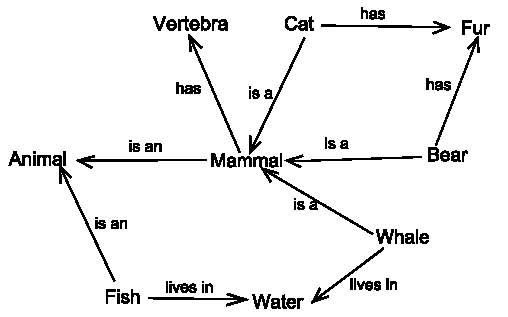
\includegraphics[width=0.48\textwidth]{img/semantic-network}
  \caption{A semantic network from the domain of animals~\cite{semanticnetworkpict}.}
  \label{fig:semantic-network}
\end{wrapfigure}

Similarly as we classified the various types of memory by its duration and capacity, we can also differentiate memory by the type of information it retains. In 1980, N.~J.~Cohen and Squire introduced the term \textit{declarative memory}~\cite{cohen1980preserved}. Declarative memory retains the conscious memory, this involves mainly events and facts. Another type of memory is called the \textit{procedural memory} and is the type of memory we are not consciously aware of and which makes humans capable of the acquisition of both the motor and cognitive skills. For example riding a bike or swimming are tasks that are learned and collected as procedural memories~\cite{MichaelW.Eysenck2008}.

The declarative memory can be further classified into the \textit{episodic memory} and the \textit{semantic memory}. The episodic memories are memories that store information associated with a specific event whereas the semantic memories include the knowledge of the meanings of words, factual information and encyclopedic memories~\cite{cohen1980preserved}. In the human brain, semantic memories seem to be organized hierarchically, i.e. if we acquire the information, that Husky is a dog, our brain automatically infers that it has fur, four legs, two ears, it must eat to stay alive, and so on~\cite{mcclelland1995there}. This representation of semantic relation between concepts is called a \textit{semantic network}. An example of a semantic network is illustrated on Figure~\ref{fig:semantic-network}.

\section{The Science of Learning}
\label{science-of-learning}

Throughout the last one hundred years, researchers have been trying to figure out the complex cognitive processes in the human brain, which are responsible for our ability to learn~\cite{RichardE.Mayer2010}. So far, we have explored human memory from its structural, organizational and functional point of view. In this chapter we look at memory and learning from the perspective particularly relevant in education and educational systems. Our objective is to understand how to present material in ways to help people learn, i.e.~increase their motivation, the speed of learning and reduce the need for repetition caused by forgetting.

In a book called \textit{Applying the Science of Learning} by Richard~E.~Mayer, a professor of psychology at the University of California, the science of learning is organized into the following three components:

\begin{itemize}
  \item The Science of Learning
  \item The Science of Instruction
  \item The Science of Assessment
\end{itemize}

All of these components are to some extent related to our research. However, the science of learning is the most related since it concerns human memory and learning. The science of instruction is about the manipulation of the student's environment in order to foster learning, it's the scientific study of how to help people learn. In educational systems, this is usually done by incorporating \textit{instructional policies}, the strategies or a set of instructions that help students maintain engagement and increase the amount gained knowledge in one session. Instructional policies guide students during learning by e.g. the selection of appropriate questions or the number of options in multiple-choice tests. Lastly, the science of assessment seeks to determine what people know, which is important so that we are able to quantify the effectiveness of different instructional methods~\cite{RichardE.Mayer2010}.

\subsection{Self-regulated Study}
\label{study}

An important aspect of learning and self-regulated study is the ability to choose the most optimal methods of studying. It is sometimes hard to correctly determine how long to study or what to study and when to consider material learned. Often, people stop studying when they do not fully know the material. For example, the effect of forgetting (i.e. the loss of information) can be reduced more dramatically by the correct type of repetition. Repetition can be \textit{massed} or \textit{spaced}, in a massed presentation an item is typically revised in a short interval many times over with no intervening delay. In contrast, a spaced presentation usually consists of revisions performed across longer periods of time with delayed presentations~\cite{kornell2008learning,pavlik2007optimizing}.

Interesting fact about self-regulated study is that in situations where it is allowed to study without time limit or some different higher pressure situation, people often choose to study the most difficult items, however, under pressure people give high priority to relatively easy items. Although, in both situations, people do not study items that they think they have already learned~\cite{kornell2007promise}.

\section{Student Modeling and Memory}

Understanding the process of learning is very helpful in education and educational systems where we wish to improve student's representation. This is useful if we want to adapt our system to the needs and knowledge of individual students practicing a particular domain (e.g. the knowledge of animals, Japanese vocabulary, geography, etc.). The construction of a quantitative representation, called a \textit{student model}, is known as \textit{student modeling}~\cite{Sison1998}.

The process of learning is very closely related to the topic of our thesis as it leads to the creation of new memory. The study of learning and memory can be divided even further when we realize that we need some way to observe what students know by experiments. Thus, we cover the relevant research to student modeling and memory in three parts:

\begin{itemize}
  \item Learning
  \item Memory
  \item Performance
\end{itemize}

Although this distinction is not very important, it can help the reader better understand the underlying problem discussed in our thesis, the connection between computer science and psychology.

\subsection{Learning}
\label{learning}

Richard E. Mayer formulated learning as a change in what the student knows caused by the student's experience~\cite{RichardE.Mayer2010}. In more psychological terms, learning is the process of encoding, modifying and reinforcing information~\cite{Lewis}. For example, the encoding of the location of Portugal can be seen as learning the shape of the country, its neighbor Spain, the surrounding ocean, the fact that Portugal was part of the Roman Empire and so on.

A learning curve is the rate of the student's progress in gaining new skill or knowledge by experience in the environment (e.g. by participating in a discussion, reading a book or riding a bike). Generally, the speed of learning is proportional to the product of amount learned and amount to yet learn. This principal can be written mathematically as follows:

\begin{equation} \label{learning-differential}
  \frac{dK}{dt} = a \cdot (K_{max} - K)
\end{equation}

The coefficient $a$ in the Equation~\ref{learning-differential} represents the rate of learning. $K$ is the student's knowledge and $K_{max}$ the maximum knowledge possible. Several functions modeling the learning curve were proposed in the past, namely the power law, exponential and hyperbolic function. Most researchers nowadays believe that learning follows the power law~\cite{Klusasek2014}.

\begin{figure}[htbp]
  \centering
  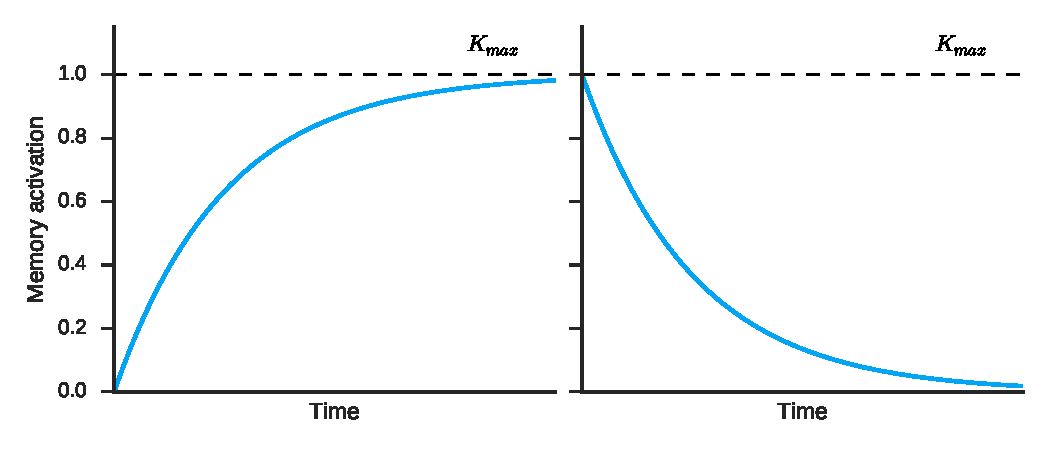
\includegraphics[width=\textwidth]{img/learning-forgetting-curves}
  \caption{Learning curve (left) and forgetting curve (right).}
  \label{fig:learning-forgetting-curves}
\end{figure}

\subsection{Memory}
\label{memory}

Memory is the biological storage that retains encoded information, for instance, the location of Portugal. The long-term memory decay is called forgetting and similarly as learning, the speed of forgetting is inversely proportional to the volume of remaining material.

\begin{equation} \label{forgetting-differential}
  \frac{dK}{dt} = -bK
\end{equation}

In Equation~\ref{forgetting-differential}, the parameter $p$ represents the rate of forgetting and $K$ is the student's knowledge of the material. Solving the differential equation yields a negative exponential. Most researchers believe that forgetting respects the power law~\cite{MichaelW.Eysenck2008}, although in some cases it is argued that exponential function with time scaled to $\sqrt{t}$ describes the phenomenon better~\cite{White2001}.

In chapter~\ref{study} we explained that a spaced presentation leads to a better and more stable long-term memory. This phenomenon is called the spacing effect and is illustrated on Figure~\ref{fig:spacing-effect}. We should also mention that our concern is only the factual knowledge which is stored as declarative memory, that is the conscious knowledge (knowing what) such as the world's countries or the English vocabulary.

\begin{figure}[htbp]
  \centering
  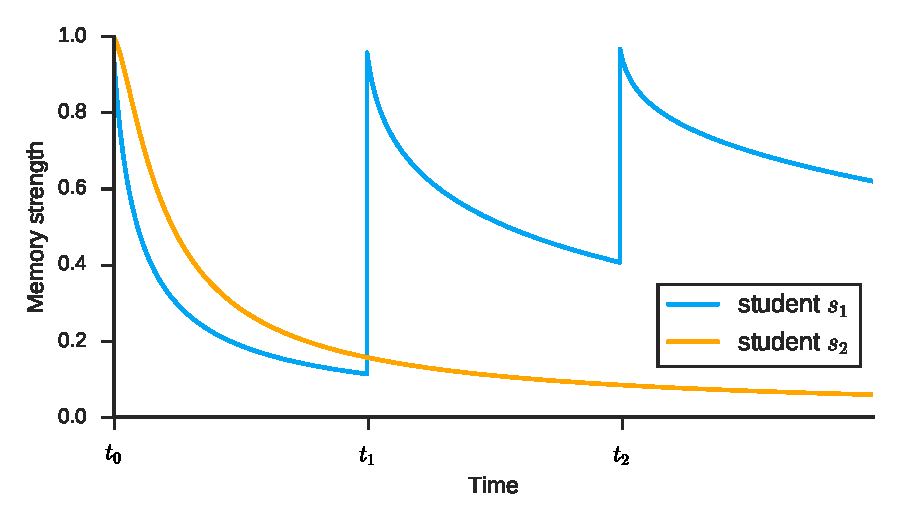
\includegraphics[width=\textwidth]{img/spacing-effect}
  \caption{Example of the spacing effect. The student $s_1$ attended three sessions at times $t_0$, $t_1$ and $t_2$ and practiced 50 items on each, the student $s_2$ attended one session at the time $t_0$ where they practiced 150 items.}
  \label{fig:spacing-effect}
\end{figure}

\subsection{Performance}

The performance of students is the determination of what they know. Performance can be estimated from the speed and precision of recall, for example by a multiple-choice test, where the correctness of answers and response time is measured~\cite{Lewis}. Performance can be seen as an instrument that describes the student's knowledge, the understanding of which is important because it helps us guide the instructional policy.

One of the most useful metric of student's performance is the \textit{memory activation} (a measurement of the ability to retrieve an \textit{item} from memory). In our case an item is any factual information that can be learned. Memory activation can be measured indirectly by observing the following attributes of students when an item is practiced:

\begin{description}[leftmargin=0cm]
  \item[Probability of recall] Probability of the student recalling the practiced item, this can be measured as the fraction of the number of successful recollections and the number of all presentations.
  \item[Latency of recall] Latency of the student when retrieving the practiced item from memory. Latency of recall can be measured by observing the response times of students.
  \item[Savings in relearning] The number of required revisions of the practiced item in order to fully regain its knowledge~\cite{MichaelW.Eysenck2008}.
\end{description}

We can further distinguish the following levels of learning as measured by memory activation (portrayed on Figure~\ref{fig:knowledge-levels}):

\begin{figure}[htbp]
  \centering
  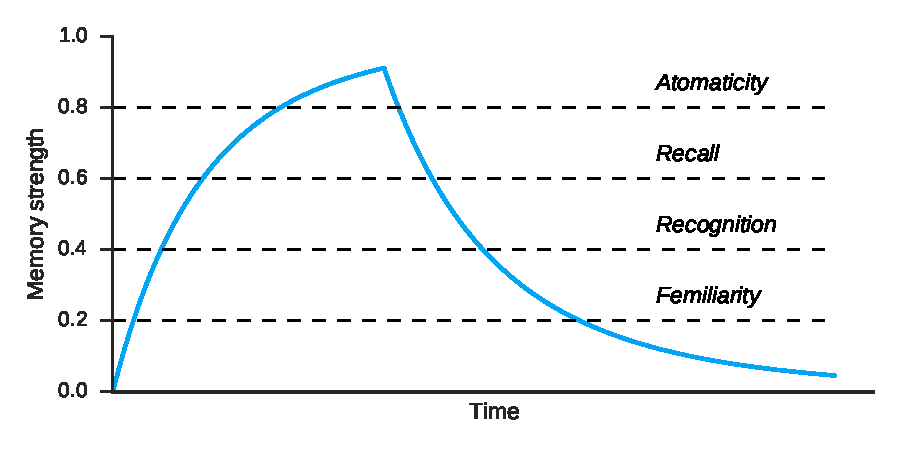
\includegraphics[width=\textwidth]{img/knowledge-levels}
  \caption{Levels of learning~\cite{Lewis}. The line indicates a simplified example of the progress of student's knowledge. Study time takes place between the times $t_0$ and $t_1$, this is followed by the post-study time.}
  \label{fig:knowledge-levels}
\end{figure}

\begin{description}[leftmargin=0cm]
  \item[Familiarity] The student has feeling they knew the item in the past but cannot remember anymore.
  \item[Recognition] The student recognized the item when presented multiple-choice options but could not remember otherwise.
  \item[Recall] The student is able to recall the item with some effort. Note that in cognitive science we distinguish \textit{free recall} and \textit{cued recall}. Free recall is the ability to remember an item without any help (e.g. recalling the name of a country), in the case of cued recall, we are given an information which can help us remember (e.g. first letter of the country we are to remember).
  \item[Automaticity] The student recalls the item instantaneously when presented. Note that the level of automaticity can be measured by the latency of recall.
\end{description}

\section{Relevant Student Models}
\label{relevant-models}

In this section we discuss the models relevant to our work. There are two main components that concern us and we can treat them independently, the first is the estimation of probability that a student knows an item before they answer the very first question about the item. The second is the estimation of the current knowledge of a student which combines the prior knowledge and the knowledge they acquired as they practiced~\cite{Papousek2014}.

\subsection{The Logistic Function}

We begin with the equation of the sigmoid logistic function, which is used for prediction of correct performance in all of the following models.

\begin{equation} \label{eq-sigmoid}
  \sigma(m) = \frac{1}{1 + e^{-m}}
\end{equation}

Equation~\ref{eq-sigmoid} shows the sigmoid function $\sigma : \mathbb{R} \rightarrow \mathbb{R}$ with argument $m$ representing memory activation. If $m = 0$, the probability of correct performance is $0.5$.

In the case of multiple-choice questions we also want to take into account the probability that a student guesses the correct answer. This can be done by introducing the argument $r$ representing the ratio of the number of correct answers and all possible answers, for instance $r = 1/6$ if there are exactly 6 options while only 1 option is correct. The modified version of the sigmoid function is depicted in Equation~\ref{eq-sigmoid-r}.

\begin{equation} \label{eq-sigmoid-r}
  \sigma(m, r) = r + \left(1 - r\right)\frac{1}{1 + e^{-m}}
\end{equation}

Note that $\sigma(m, 0) = \sigma(m)$. The shape of such logistic function is shown in Figure~\ref{fig:sigmoid-function}.

\begin{figure}[htbp]
  \centering
  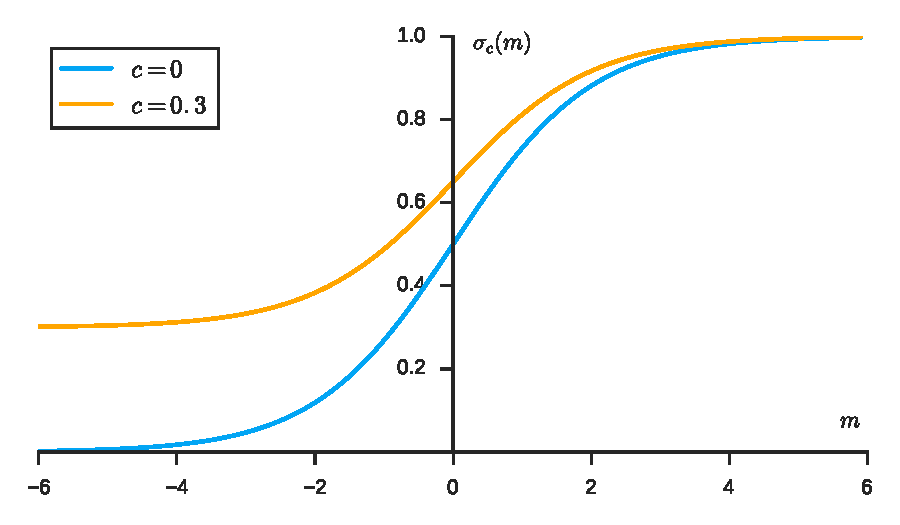
\includegraphics[width=\textwidth]{img/sigmoid-function}
  \caption{Comparison of sigmoid functions $\sigma(m, r)$ with two different values of the argument $r$.}
  \label{fig:sigmoid-function}
\end{figure}

\subsection{Elo System}
\label{elo}

Elo rating system and its extension Glicko are very popular mathematical models~\cite{rotou2015ranking} used in competitor-versus-competitor games such as chess where the goal is to rate players with scores according to the number of opponents they defeated or were defeated by while also honoring each player's skill~\cite{Vanek2014}. Recent research has shown that Elo system is also suited for student modeling and it was previously very successfully adopted for the estimation of prior knowledge of students~\cite{Niznan2015}.

In the adopted version of Elo system we have the student's skill $\theta_s$ and the difficulty of an item $d_i$. Equations~\ref{eq-elo-skill} and~\ref{eq-elo-difficulty} demonstrate an update of the student's skill and the item's difficulty after one answered question. The parameter $R$ is $0$ or $1$ depending on the correctness of the student's answer. The probability that a student $s$ with a given skill $\theta_s$ will answer correctly on the presented question of difficulty $d_i$ is estimated by a logistic function in~Equation~\ref{eq-elo-logistic}.

\begin{equation} \label{eq-elo-logistic}
  P(R = 1|s,i) = \sigma(\theta_s - d_i)
\end{equation}

\begin{equation} \label{eq-elo-skill}
  \theta_s \gets \theta_s + K(R - P(R = 1|s,i))
\end{equation}

\begin{equation} \label{eq-elo-difficulty}
  d_i \gets d_i - K(R - P(R = 1|s,i))
\end{equation}

The constant parameter $K$ affects the change in the estimates $\theta_s$ and $d_i$. Higher value means faster change after few questions, in contrast lower value makes the change slower. This is a problem in cases where the number of answers varies over time. It has been demonstrated that the use of an uncertainty function $\frac{\alpha}{1 + \beta n}$, which considers the number of answers of students in the system, makes the predictions more stable and increases accuracy~\cite{Vanek2014}.

\subsection{Performance Factor Analysis}
\label{pfa}

Performance Factor Analysis (PFA) is a student modeling approach based on the Learning Factor Analysis (LFA)~\cite{Pavlik2009,cen2007over}. Memory activation in the PFA model can be seen as the sum of the item's difficulty and all student's answers with estimated weight for successful and unsuccessful answer. The standard PFA equation is formulated with the incorporation of knowledge components (KCs), which may include skills, concepts, facts, or any fragment of a domain-specific information that should be used to accomplish a task~\cite{vanlehn2006}. In our work, we use PFA and its extensions for the estimation of current knowledge.

\begin{equation} \label{eq-pfa-standard}
  m(i,s,f) = \sum_{j \in KCs} \beta_j + \gamma_j s_{i,j} + \delta_j f_{i,j} 
\end{equation}

\begin{equation} \label{eq-pfa-standard-p}
  P(m) = \sigma(m)
\end{equation}

In Equation~\ref{eq-pfa-standard}, where $m$ is a function of the student's knowledge of item $i$, the parameter $\beta_j$ is the difficulty of the knowledge component $j$. The counts of current successes and failures of the practiced item $i$ and the knowledge component $j$ are represented by $s_{i,j}$ (number of successes) and $f_{i,j}$ (number of failures), where $\gamma_j$ and $\delta_j$ give a weight to each success and failure. An item is retrieved only if its memory activation $m$ is above certain value, e.g. if $m = 0$, we can calculate from Equation~\ref{eq-pfa-standard-p} that the probability of correct performance is $0.5$.

\subsection*{The Elo/Extended Version}
\label{pfae}

The standard PFA model is defined in terms of knowledge components which is not always needed. The main disadvantage, however, is the inability to consider the order of answers. Another problem with the standard PFA model is that it does not take into account the probability of guessing~\cite{Papousek2014}. Both of these issues are solved by the adjustments depicted in Equation~\ref{eq-pfa-extended}.

\begin{equation} \label{eq-pfa-extended}
  m \gets \begin{cases}
            m + \gamma \cdot (1 - P(m)), & \text{\textbf{if }} \text{the answer was correct} \\
            m + \delta \cdot P(m), & \text{\textbf{otherwise}}
          \end{cases}
\end{equation}

\begin{equation} \label{eq-pfa-standard-p}
  P(m) = \sigma\left(m,\frac{1}{n}\right)
\end{equation}

The initial value of $m$ can be estimated from the Elo model which was discussed in chapter~\ref{elo}, i.e. $m = \theta_s - d_i$. The variable $n$ in the Equation~\ref{eq-pfa-standard-p} represents the number of options in multiple-choice question. The probability of guess is thus $\frac{1}{n}$. Note that this is a simplification as it does not consider the possibility that a student answers correctly only by ruling out some portion of the other displayed options (in which case they do not know the correct answer even though there is higher chance of guess)~\cite{Pelanek2015a}.

To get a better idea of how this model works, suppose that a new student $s$ decides to practice autonomous communities of Spain. Before the first question about any item is presented, the memory activations of all items in the system are estimated from the Elo model, i.e. $m = \theta_s - d_i$ for each student $s$ and item $i$. Now, the system can select an appropriate question for the student, this is often based on the probability of correct performance $P(m)$. After the student $s$ answers the presented question, the memory activation $m$ of the autonomous community $i$ is locally updated for the student $s$ depending on correctness of their answer. In the next repetition of the same item, the updated memory activation of the student is used again for the estimation of correct performance and updated subsequently. This process is repeated for each answered item.

\subsection*{The Decay Factor}
\label{pfag}

Another variation of the original PFA model was proposed by Yue Gong~\cite{Gong2011}. The idea of the model is based on the fact that we expect the student who answered in four presentations two times correctly in the last two presentations to perform better than the student who answered correctly in the first two presentations. The extended model introduces a decay factor $\xi$ that changes the behavior of the parameters $s_{i,j}$ and $f_{i,j}$ by penalizing the older answers. The modifications are shown in Equations~\ref{eq-pfa-gong-s} and \ref{eq-pfa-gong-f}.

\begin{equation} \label{eq-pfa-gong-s}
  s_{i,j} = \sum_{k=1}^{n} y_k \cdot \xi^{n-k}
\end{equation}

\begin{equation} \label{eq-pfa-gong-f}
  f_{i,j} = \sum_{k=1}^{n} |y_k - 1| \cdot \xi^{n-k}
\end{equation}

The variable $y_k$ represents the correctness of the $k$-th question. For example, suppose that a student was presented with a question in five trials, suppose that the student answered incorrectly in the first three trials and answered correctly in the last two. Now for the given value of $\xi = 0.8$ we can calculate the values of $s_{i,j}$ and $f_{i,j}$. Equation~\ref{eq-pfa-gong-example} demonstrates the result of such scenario where we see that the weight of all successes surpasses the weight of all failures.

\begin{equation} \label{eq-pfa-gong-example}
  \begin{split}
  s_{i,j} & = 0 \cdot 0.8^4 + 0 \cdot 0.8^3 + 0 \cdot 0.8^2 + 1 \cdot 0.8^1 + 1 \cdot 0.8^0 \\
  & = 1.8 \\
  f_{i,j} & = 1 \cdot 0.8^4 + 1 \cdot 0.8^3 + 1 \cdot 0.8^2 + 0 \cdot 0.8^1 + 0 \cdot 0.8^0 \\
  & = 1.56
  \end{split}
\end{equation}

The problem of this model is that it cannot be straightforwardly adjusted so that it includes the probability of guessing, particularly in cases where the practices were presented in the form of multiple-choice questions with varied number of options.

\subsection{Models of Forgetting}
\label{spacing-effect}

So far, all the presented models did not account for the effect of forgetting. Although the use of a decay factor can be seen as a way to penalize past answers, it does not consider intervals of time between repetitions of an item. In the ACT-R (Adaptive Character of Thought--Rational) modeling system~\cite{Pavlik2003}, the memory activation $m$ of a student is a function of prior practices. This function does not account for correctness of prior answers or their difficulty, it considers only counts and times of past repetitions.

\begin{equation} \label{eq-actr}
  m(\mathbf{t}) = \ln{\sum_{i=1}^{n} t_{i}^{-d}}
\end{equation}

The memory activation function used in ACT-R model is shown in Equation~\ref{eq-actr}, the argument $\mathbf{t}$ is a vector of seconds that passed since each of the $n$ repetitions were performed by a student. The parameter $d$ represents memory decay (the speed of forgetting). Note that the equation is just a simplification of the reality and does not take into account many very important aspects of forgetting, e.g. the mentioned spacing effect.

An item will be retrieved only if its memory activation is above certain threshold. In ACT-R model, the probability of recall is given by the value of the threshold $\tau$ and the measure of noise $s$: 

\begin{equation} \label{eq-actr-p}
  P(m) = \sigma\left(\frac{\tau - m}{s}\right)
\end{equation}

Philip~I.~Pavlik and John~R.~Anderson~\cite{Pavlik2005} developed an extended version of the equation in which the decay is a function of the activation at the time the item was presented. The Equations~\ref{eq-pavlik-decay} and~\ref{eq-pavlik-activation} demonstrate the replacement of the parameter $d$ with a recurrent function $d_i$ that depends on the past timing distances between presentations.

\begin{equation} \label{eq-pavlik-decay}
  d_i = ce^{m_{i-1}} + a
\end{equation}
\begin{equation} \label{eq-pavlik-activation}
  m(\mathbf{t}) = \ln{\sum_{i=1}^{n} t_{i}^{-d_i}}
\end{equation}

The parameter $c$ affects the impact of the spacing effect while the parameter $a$ affects the slope of the decay. Since $m_0 = -\infty$, the value of $d_i$ is always equal to $a$ at the first student's practice of an item. Instinctively, when $c = 0$, the result of the equation is equivalent with the Equation~\ref{eq-actr}. Because the computation is recursive and a bit complex, we present the pseudo-code of the algorithm computing the memory activation function (see Algorithm~\ref{alg-memory-activation}). Note that the time complexity of the function is $\mathcal{O}\left(\frac{n(n-1)}{2}\right)$.

\begin{algorithm}
  \caption{The function $\textsc{MemoryActivation}: \mathbb{N}^n \rightarrow \mathbb{R}^n$ takes the vector $\mathbf{t}$ in descending order, e.g. $[56800, 56400, 3600, 60, 0]$ (the last zero is the current practice). The result of the computation is a vector $\mathbf{m}$ of student's memory activations during each practice.}
  \label{alg-memory-activation}
  \begin{algorithmic}[1]
    \Function{MemoryActivation}{$\mathbf{t}$}
      \State $n \gets \mathit{dimension}(\mathbf{t})$
      \State $m_0 \gets -\infty$
      \For{$i \gets 2$ \textbf{to} $n$}
        \State $s \gets 0$
        \For{$j \gets 1$ \textbf{to} $i-1$}
          \State $d_j \gets ce^{m_{j-1}} + a$
          \State $s \gets s + (t_j - t_i)^{-d_j}$
        \EndFor
        \State $m_i \gets \log(s)$
      \EndFor
      \State \Return $\mathbf{m}$
    \EndFunction
  \end{algorithmic}
\end{algorithm}

The purpose of this adjustment is to address the spacing effect by extending the ACT-R's activation equation. The experiments done by P.~I.~Pavlik and J.~Anderson showed better fits and less variations in parameters. However, the experiments were performed in controlled environment on students who had no prior knowledge of the material they were practicing (Japanese vocabulary)~\cite{Pavlik2005}. In domains where the students differ in their age, education and the prior knowledge of the practiced material, the parameters might be very unstable or even impossible to estimate.
